\documentclass{article}
\usepackage[utf8]{inputenc}
\usepackage[english]{babel}
\usepackage{graphicx}

\setlength{\parindent}{4em}
\setlength{\parskip}{1em}

\title{Missing data: a simple introduction}
\author{Marius Dioli}
\date{February 2019}

\begin{document}
	
	\maketitle
	
	
	\section{Introduction}
	... ''eng and Romero (2003), Xie and Meng (2012)). In general,
	the problem of multiphase inference can be formulated as one of missing data. However, in the
	multiphase setting, missingness arises from the preprocessing choices made, not a probabilis
	tic response mechanism. Thus, we can leverage the mathematical and computational methods
	of this literature, but many of its conceptual tools need to be modified. Multiple imputation ad
	dresses many of the same issues as multiphase inference and is indeed a special case of the
	latter. Concepts such as congeniality between imputation and analysis models and self-efficiency
	(Meng ( 1994)) have natural analogues and roles to play in the analysis of multiphase inference
	problems.''
	
	In this paper we will focus on the Multiple Imputation in the context of correcting for missing data before analysis. Blocker and Meng argue that general preprosessing can be evaluated in the missing data paradigm, but this is outside the scope of this paper. We refer readers to Block and Meng for an in depth consideration of the subject.
	
	The public database is perhaps the context where MI is most useful. These are often analyzed by multiple users with varying degrees of statistical knowledge and resources. All public databases have missing data, and typically users do not have the knowledge to deal with missing data satisfactoraly. Even if they do, the database constructors often have more information about the missing data than the end user, and so can better compensate for this.
	%TODO Introduce the concept of multiphase inference. Reference meng2017 and Blocker and meng
	If one is to do anything of import in science, one has to manipulate and analyze data. However, due to a variety of factors, data is often flawed. One major flaw one can have, and the topic of this thesis, is missing data. The consequence of missing data is always a reduction in efficiency and may also lead to bias.
	
	//A variety of ad hoc approaches are commonly used to deal with missing data, and many of the techniques described in this thesis are either//
	
	//This thesis will approach the problem of missing data from the bayesian perspective and with the goal of imputing or removing data. Other methods motivated from the frequentist perspective such as likelihood based methods will be touched on breifly as alternatives. The strength of the bayesian approach is that it provides a principled way to account for uncertainty about the missingness mechanism and the true distribution of the full data. //
	
	To quote MENG: ''imputation is not (merely) a compu-
	tational tool but rather a mode of inference, which al-
	lows hierarchical and sequential input of assessment
	and information'' [Multiple-Imputation Inferences with Uncongenial Sources of Input]
	
	
	//Missing data is almost always considered in the context of fitting a model or making inference.//
	
	.. We will measure its efficacy on synthetic data and real data before comparing it with an alternate method that is gaining in popularity, machine learning.
	
	This paper is by no means comprehensive, but strives to give the reader a proper introduction to the problem of missing data and the technique of multiple imputation.
	// fyldig
	
	As detailed in Xie and Meng [DISSECTING MULTIPLE IMPUTATION FROM], much of modern data analysis is done in a multi-phase paradigm, where the distinct and sequential phases data acquisition, data pre-processing, and data analysis, can have different or even contradictory assumptions.
	

	
	\section{Terminology and basic missingness theory}
	In the following section I will mostly adhere to the notation of Rubin in (citation), as it is both well established and quite general. However, I will adapt it slightly by using the observed/missing notation in (missing data) for readability, as it is easier for an unfamiliar audience and non-specialists to understand.
	
	\subsection{What is missingness?}
	When we say a variable is missing we mean that we have not observed it. The variable still has a value, but this value is hidden from us for some reason. What this reason might be will be described in detail later in this section. By treating missingness as a probabalistic phenomenon, statistically rigorous tools for dealing with it become available. 
	
	Let $Y=(y_{ij})$ be a $nxk$ complete data matrix (i.e. with no missing values), with the ith row $y_{i}=(y_{i1}, ..., y_{ik})$ where $y_{ij}$ is the value of variable $Y_{j}$ for unit $i$. Let also the missingness indicator matrix $M = (m_{ij})$ be an $nxk$ such that $m_{ij} = 1$ if $y_{ij}$ is missing and $m_{ij} = 0$ if $y_{ij}$ is observed. Both $Y$ and $M$ are random variables, and we assume for simplicity that the rows $(y_{i}, m_{i})$ are independent and identically distributed over i. It is possible to have more than two possible values for each entry of the $M$, for example when we wish to differentiate between different kinds of non-response. However, we will not explore this in this paper. Now, given $m_{i}$, we can partition $y_{i}$ into $y^{o}_{i}$ and $y^{m}_{i}$, corresponding to the components that are observed and missing respectively (where the corresponding entry in $m_{i}$ is 0 or 1 respectively).
	
	\subsection{The missingness mechanism}
	
	The missingness mechanism is characterized by the conditional distribution of $m_{i}$ given $y_{i}$, i.e. $f_{M|Y}(m_{i}|y_{i}, \theta)$, where $\theta$ denotes unknown parameters. Stated differently the missingness mechanism is the probability of data being missing given the values of Y, missing and observed. 
	
	The missingness pattern in $Y$ does not matter for the following definitions, and can be any of the following: *(Figure from page 9 Rubin)* 
	However, the missingness pattern will affect the efficacy of methods used to deal with missingness, and we shall explore this in subsequent sections.
	
	We distinguish between three different missingness mechanisms by considering how $M$ is related to $Y$: Missing Completely at Random (MCAR), Missing at Random (MAR), Missing Not at Random (MNAR). These can be roughly thought of as being in order of strictness from strictest (MCAR), to least strict (MNAR). Rubin(1976) [missing data book] introduced these missingness mechanisms, and they determine which techniques are appropriate to use on a given problem. **These mechanisms are rarely the case in practice, but it will be shown later that assuming them is reasonable in many circumstances. **
	
	\textbf{Missing Completely At Random (MCAR)}:
	This kind of missingness occurs when, $\forall i$ and any distinct values $y_{i}, y^{\ast}_{i}$ in the sample space of Y, $f_{M|Y}(m_{i}|y_{i}, \theta) = f_{M|Y}(m_{i}|y^{\ast}_{i}, \phi)$. In other words, it means that the probability of missingness is independent of both the observed and the missing data, and we can view the observed data as a random sample of the complete data.
	
	\textbf{Missing At Random (MAR)}:
	In this case, $\forall i$ and any distinct values $y^{m}_{i}, y^{m\ast}_{i}$ in the sample space of $y^{m}_{i}$, $f_{M|Y}(m_{i}|y^{o}_{i}, y^{m}_{i}, \theta) = f_{M|Y}(m_{i}|y^{o}_{i}, y^{m\ast}_{i}, \theta)$.
	This means that the probability of missingness, conditioned on the observed data, is independent of the missing data. Assuming MAR is less restrictive than MCAR, and may be considered a more plausible assumption about missing data in many contexts. 
	
	\textbf{Missing Not At Random (MNAR)}:
	If the above equation does not hold for some $i$ and some $y^{m}_{i}, y^{m\ast}_{i}$, then the missingness mechanism is called missing not at random (MNAR). This means that the probability of missingness is dependent on the missing data even after conditioning on the observed data.
	
	
	\subsection{Illustrative example}
	
	The following example illustrates the three different types of missingness.
	
	Suppose you are doing a study in which you want to investigate people's sleep patterns. You send N people a survey asking them for the average amount of sleep they got each night in 2018. You send a follow-up survey for 2019. Table 1 shows simulated data for N = 15 people drawn from a bivariate normal distribution with $\mu_{x} = \mu_{y} = 7.5$, $\sigma_{x} = \sigma_{y} = 2$, and a correlation $\rho = 0.4$. The first two columns show the complete data for X and Y, while the other three columns show the values for 2019 after imposing missingness by three methods.
	
	\begin{figure}
		\centering
		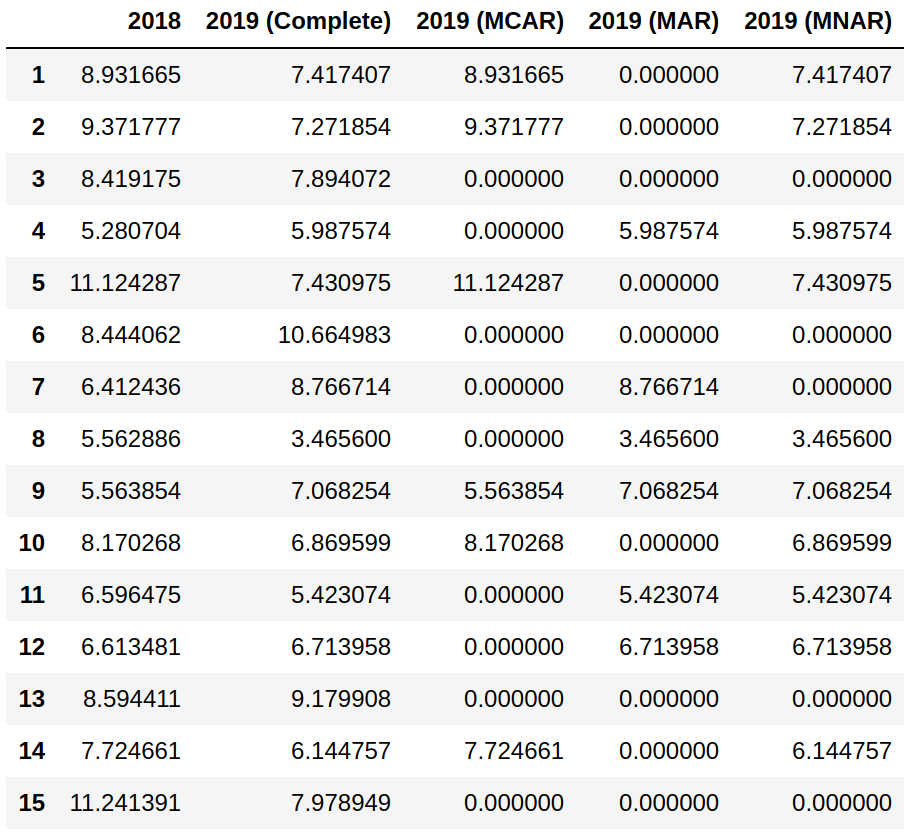
\includegraphics[width=\linewidth]{missingness}
		\caption{Different missingness mechanisms}
		\label{fig:miss1}
	\end{figure}
	
	In the MCAR scenario, we see a random spread of missing data, i.e. a random subset of those who answered the 2018 survey also answered the 2019 one. Things get more interesting in the next two columns. Suppose you are only interested in those who've slept less than 7.5 hours on average, so you only send a follow-up survey to those who reported less than 7.5 hours of sleep for 2018 (2018<7.5). This is MAR, since the missingness of the 2019 entries depends on the values for 2018. For the final column, suppose you sent out your 2019 survey to all the individuals who answered the 2018 one, but include a line stating "Only answer this survey if you slept less than 7.5 hours on average in 2019" (2019 < 7.5). This is MNAR, since the missingness of the 2019 entries depends on the values for those entries. Remember, the full dataset exists, but it has been censored due to some mechanism, in this case through your own design. 
	
	
	\subsection{The validity of missingness mechanisms}
	
	In controlled environments, like the one from our example, we can guarantee that data are MAR since we control the censoring of the data (in this case by placing a cutoff between 2018 and 2019). However, it is rare that we have this much control over our data, and a compelling reason to censor it so. In most real world scenarios we only have the data at hand to inform us about the missingness mechanism. Unfortunately, we cannot infer the missingness mechanism from data.  We can check the validity of MCAR against MAR, but only under the unverifiable assumption that the data is not MNAR. Neither can we use the data at hand to support or refute on specific MNAR mechanism over another. The literature stresses the importance of sensitivity analyses in this case, checking the sensitivity of our inference under a variety of plausible assumptions. Finally MAR cannot be checked empirically against MNAR  (Cite from page 8, 9, and 10 in missing data). We therefore have to assume the missingness mechanism, most often MAR, and there are strong arguments for this. First and foremost is that assuming MAR yields good empirical results, which will be shown in later sections. %TODO Add more reasons for assuming MAR
	
	\section{Imputation}
	
	\subsection{What is imputation?}
	Imputation refers to substituting or ''filling in'' of missing values with plausible estimates.The main strength of imputation is that it does not change the nature of the subsequent analysis. It makes it much easier for the data processor and analyst to work together since the processor's techniques won't interfere with the analysts'. This is, at least, the goal of imputation. In certain situation the information available to the imputer might differ to that available to the analyst. In such cases difficulties arise. The concept of congeniality, which we will define shortly, helps us overcome some of these difficulties. Another very practical benefit, and a strong argument for its use, is the performance gains to be had from using it. This will become clear in the experiments section.
	

	\subsection{Congeniality: when the imputer's and analysts models differ}
	As mentioned in the introduction, modern data analysis' multiple phases mean that the assumptions underlying each phase and the relationship between the phases is an important object of study.  Meng's [meng 1994] concept of congeniality provides a theoretical framework from which to evaluate these differences.
	
	
	''When the imputation model class and the (embedded) analyst’s model class
	differ, the behavior of Rubin’s rules becomes very complicated, capable of producing inconsistent variance estimators, a matter that has received recurrent
	criticisms'' [Meng 2017]
	
	Congeniality is an important concept in imputation and has a big impact on the statistical validity of MI. In short, uncongeniality arises when the analysis procedure differs substantially from the imputation model. There are many reasons for such difference, for example, the imputer might wish to include as many variables as possible to achieve an accurate imputation, while the analyst might be interested in only a subset of the covariates and the relationship between these. However, as Meng [1994] states, ''If the imputer's model is reasonably accu-
	rate, then following the multiple-imputation recipe
	prevents the analyst from producing inferences with
	serious nonresponse biases''
	
	
	
	\subsection{Does imputation yield valid inference?}
	Techniques are baased on the bayesian paradigm, but 
	
	Rubin (1996) defines 
	
	
	\subsection{Techniques of interest}
	To properly evaluate the performance of MI, we should compare it to other similar and commonly used techniques, i.e. techniques that manipulate the dataset by either imputing or removing values. When choosing to apply a method it is important to keep two questions in mind. First, does the method under consideration give us consistent estimators for our model? Second, does the method give us appropriate measures of precision? How the following methods answer these questions is how we will decide the superiority of one method over another.
	
	There are two other competing methods which we should touch on briefly before continuing. Weighting procedures and likelihood-based methods are ... alternatives to multiple imputation. However, there is reason to prefer MI as the default options over these for a few reasons. First that, given congeniality, MI tends to outperform likelihood-based methods for small sample sizes, while delivering similar performance for large sample sizes \cite{schafer_multiple_2016}.
	
	\subsection{Ad hoc methods}
	This section is mostly adapted from Carpenter and Kenward [Ch2.5 missing data]. Although Ad hoc is pejorative in certain circumstances, it is used here to indicate that the methods below are motivated by convenience rather than any methodological concern.
	
	\textbf{Case deletion, also called complete case analysis (CCA):}
	Probably the most common technique in use for dealing with missing data, CCA involves restricting analysis to entries with complete data. For those familiar with programming, a typical example would be to remove all rows from a dataframe with NaN entries. The first and most obvious problem with this approach is that it drastically reduces the amount of useable data. This holds an intuitive appeal, as it is both exceedingly simple to implement, and seem to have the regrettable but sometimes minor effect of lower accuracy. However, depending on the missingness mechanism, this might be wrong, and can actually introduce bias into the data. For example, suppose you want to find the mean and standard deviation in the height of a population. If for some reason you lack all entries for people above 200cm, then disregarding these missing entries in a CCA will lead to biased estimates for both the mean and variance. An implicit assumption, therefore, of CCA is that the observed data is a random sample of the underlying distribution. This means that CCA implicitly assumes MCAR, and we see in [schafer and graham] that we get unbiased inference in this scenario, if with lower accuracy depending on the amount of missing data. However, as with the height example, deviation from MCAR can introduce bias. See Schafer and Graham, ... for examples of how inference is affected. (CITE REVIEW PAPER FROM TURID). 
	
	\textbf{Mean imputation:}
	Another common practice, this technique involves substituting the missing values with the mean of the observed values for that variable. As stated in Schafer and Graham [2002], this has the effect of preserving the mean of the distribution one wishes to draw inference about, but distorts other parameters such as variance and covariance. Covariance especially is distorted due to mean imputation taking only the varible under consideration as input. In addition to this the technique breaks down when confronted with categorical variables where the mean does not exist (and it is clear how a majority vote imputation might skew the data). %Add some more math from either schafer and graham or another source
	
	
	\textbf{Last Observation Carried Forward (LOCF):x}
	This method is mostly used in longitudinal studies where individuals drop out, withdraw, or are lost over the course of the studies. LOCF involves imputing the missing values for an individual with the last observed value for that individual. Leaving aside questions of precision, LOCF produces biased estimators in all except very specific MNAR circumstances (Kenward and Molenberghs 2009 get article). With LOCF we are effectively assuming that for each individual that drops out their responses do not change at all for the remainder of the study, a highly unrealistic assumption. It can be concluded, therefore, that LOCF is the worst imputation method of those mentioned here, and all the other methods are preferable. According [Missing data] "LOCV is neither valid under general assumptions nor based on statistical principles, it is not a sensible method, and should not be used".
	
	\textbf{Regression:}
	Regression imputation functions by regressing the variable(s) with missing entries on the fully observed variables, or subsets that are fully observed. To illustrate this, let us consider the simplest case, with one fully observed variable $x$ linearly related to a variable with missing data $y$. Fitting a regression of $y$ on $x$, we have$$Y_{i} = \beta_{0} + \beta_{1}x_{i} + \epsilon \qquad i\in(0,...,n)$$ obtaining estimates of the regression parameters $\hat{\beta_{0}}$ and $\hat{\beta_{1}}$ allows us to impute $E(y_{i}) = \hat{\beta_{0}} + \hat{\beta_{1}}x_{i}$. This is the best of the ad hoc methods, as it gives us much more plausible imputations that can vary. However, even in this simple case it yields imputations that tend to be less variable than the observed data. Therefore, using them in inference will most often lead to underestimated standard errors and p-values. If there are non-linear relationships in the data, this method's performance breaks down with regard to other aspects of inference as well.
	
	For more in depth descriptions and examples of these methods we refer the reader to [missing data handbook].
	
	\subsection{Statistically principled methods}
	The bayesian paradigm is ideal for more statistically principled imputation, as it allows us to effectively model the unknown given the known, and makes assumptions explicit.
	
	\textbf{Single imputation}
	To build our intuition about multiple imputation it is relevant to discuss the single imputation case, and how its shortcomings are rectified in MI.
	
	\section{Multiple imputation}
	One sizeable weakness of the earlier imputation methods is that they use points as estimates of distributions. Hence, subsequent measures of precision are biased downwards. Multiple imputation solves this problem by creating multiple imputed datasets drawn from a posterior distribution and then combines them in the final step. This preserves the distributional variation in the missing data, and 

	
	
	Multiple imputation can be thought of as three distinct steps:
	1) M imputed datasets are generated
	2) The intended analysis is performed separately on all M datasets
	3) The results of the analysis are combined using Rubin's or Meng's rules to create a single MI result.
	
	Highly robust technique that yields gains even with relatively small portions of missing data. It has only reached desired levels of performance in the last decade due to the computing power required. 
	
	Bayesian approach. Although MI is motivated from the Bayesian perspective, much of today's inference whether in science or industry is dominated by frequentist analyses. This causes some (Reference Fay and stuff from MENG) to question whether inference under MI is valid at all. To address this Meng [1994] developed the concept of congeniality, which we will go into more detail on soon.
	
	Between imputation variance and within imputation variance
	
	
	While MI is motivated from the bayesian perspective, it is most often used with subsequent frequentist inference. Thus ...
	
	\subsection{Specifying the imputation model}
	
	
	We often want to include as many covariates as possible. X have shown that even mildly correlated auxiliary variables can improve subsequent inference [cite annotadet article]. However, this can cause the imputation and and analyses models to be uncongenial.
	
	\subsection{Rubin's rules and Meng's adaptations}
	
	Under congeniality, Rubin's rules for calculating standard errors, parameter values, and variance suffice.
	
	If models are uncongenial, we use Meng's rules.
	
	\subsection{Potential pitfalls and criticism}
	The following arguments apply for imputation in general, but we will consider them in the context of MI. When there is missing data in several variables of different types ,for example continuous and binary, and the data is structured, specifying the imputation model can be quite difficult. This is because it has to be a joint model...
	
	
	. Among all the
	criticisms of multiple imputation, the recent work
	of Fay (1991, 1992) is the most intense, as it is
	directed at the validity of multiple-imputation in-
	ference in practice. Fay provided several examples
	(see also Kott, 1992) to show that the variance esti-
	mator obtained from the repeated-imputation combining rules disagrees asymptotically with the sam-
	pling variance of the repeated-imputation estimator,
	even when the imputation model is correctly speci-
	fied. [MENG]
	
	%^fixed with congeniality
	
	Taking all this into account, it is important to see MI in context of the options available to someone working with data. As we have established earlier, simply ignoring missing data can lead  to serious biases, while alternative methods yield similar if not inferior performance in certain cases. As long as a potential user is aware of the potential pitfalls, MI is the superior method for dealing with missing data.
	
	
	\subsection{When to use multiple imputation?}
	Computational resources and time to create the full joint imputation model. (Handbook 236)
	
	A common measure used to decide when to use multiple imputation is percentage of missing data.
	
	However, Madley-Dowd et. al. (Proportion of missing data paper) propose a different measure.
	
	MI can be used to perform sensitivity analysis by varying the imputation model.
	
	\section{Experiments}
	In this section we will use Madley-Dowd et. al.'s missingness measure to...
	
	\subsection{MICE}
	''The
	increased flexibility in modeling these conditional distributions may outweigh
	the lack of clear theoretical justification of the method.'' Rubin
	
	We have chosen to use MICE for the experiments in this paper for two main reasons. One is the aformentioned performance and flexibility, while the other is that MICE is unlicenced and open source in contrast to other technqieus like drawing from a fully specified joint distribution found in statistical packages like STATA. In the interest of democratizing MI while retaining the desired performance, MICE was found to be superior.
	
	\subsection{Synthetic example}
	
	"The MCAR missingness mechanism
	removed the first p observations such that pn gives the
	required proportion of missing data. MAR missingness
	was simulated under a logistic regression model using
	
	The value of a was manipulated for the different simu-
	lation settings to provide the required proportion of missing
	data on average across data sets." from (P. Madley-Dowd et a)
	
	Also check out their motivation for the generating of the dataa
	
	
	In the following examples we will compare our models' performance across different data types. These are continuous, categorical (binary and multicategory), time to event data, and timeseries. The latter two 
	
	\subsubsection{Inference}
	Test statistics
	Different tests
	x
	Congenial vs uncongenial models, see the annotated paper for how they did things with regard to imputation vs analysis. 
	
	\subsubsection{Prediction}
	With large publicly available datasets on the one hand, and laws like GDPR requiring deleting certain kinds of data on the other, multiple imputation seems like a strong candidate for improving the predictive quality of models. Most of the literature focuses on inference, so there is comparatively little comparing the performance of different predictive models. Here we will compare three basic model architectures, multiple linear regression, boosted trees, and a simple neural network, to see how they perform with and without multiple imputation.
	
	
	
	
	\subsubsection{Classification}
	Like with the prediction case above, classification is an area in which the litterature on missing data is sparse and the same conditions apply. In this context we will compare logistic regression, boosted trees, and neural networks.
	
	
	\subsection{Sensitivity analysis and uncongenial models}
	
	\subsection{Real data}
	
	Description of the data
	
	HUNT Norwegian data
	
	Andreas data webSite
	balanced number of classes for classification
	
	
	\subsection{TODO}
	Difference between baysian and frequentist paradigm.
	Citation example:
	\cite[P.10]{grund_pooling_2016}.

	\bibliography{bib2}	
	\bibliographystyle{apalike}
	
\end{document}
